\documentclass[a4paper,spanish]{article}
\usepackage[spanish]{babel}
\usepackage[printwatermark]{xwatermark}
\usepackage{xcolor}
\usepackage{colortbl}
\usepackage{graphicx}
\usepackage{amsmath}
\usepackage{tikz}
\usepackage{epigraph}
\usepackage[utf8]{inputenc}
\usepackage{float}
\usepackage{hyperref}

\def\curdate{2018-08-20}
\def\documentdate{Cordoba, Argentina, 2018-08-20}
\def\distribdate{2018-08-20}
\author{%
	Mario O. Villarroel \\
	System Design/Developer\\
	\texttt{movilla@elcansoftware.com}\vspace{20pt} \\
	Pablo Giachero\\
	Product Owner\\
	\texttt{pgiachero@elcansoftware.com}
}

\usepackage{elcan}

\newwatermark[pages=1-3,color=red!50,angle=45,scale=1,xpos=0,ypos=0]{
\includegraphics{images/logo}}

\begin{document}
	\begin{titlepage}
		\noindent
		\titlefont Dise\~no WeightLogger\par
		\vspace*{15pt}
		\subtitlefont RFID control\par
		\epigraph{Este documento detalla el dise\~no para el sistema weighlogger, inclulyendo electr\'onica y Software.}%
		{\textit{\documentdate}\\ \textsc{Elcan Software}}
		\null\vfill
		\vspace*{1cm}
		\noindent
		\hfill
		\begin{minipage}{0.50\linewidth}
		    \begin{flushright}
		        \printauthor
		    \end{flushright}
		\end{minipage}
		%
		\begin{minipage}{0.02\linewidth}
		    \rule{1pt}{125pt}
		\end{minipage}
		\titlepagedecoration
	\end{titlepage}
	\section{Control de version}
\begin{elcanversions}
	\elcanversion{1.0}{Mario O. Villarroel}{}{}{\curdate} {Versión inicial}
	\elcanversion{2.0}{Mario O. Villarroel}{}{}{2018-08-28} {Traducción al español}
\end{elcanversions}

\section{Lista de distribución del proyecto}

\begin{elcandistribution}
	\distributionline {Mario O. Villarroel}{System Engineer} {movilla@elcansoftware.com} {\distribdate} 
	\distributionline {Pablo Giachero} {Product Owner} {pgiachero@elcansoftware.com} {\distribdate}
	\distributionline {Cliente Beta} {Beta tester} {cliente@elcansoftware.com}{\distribdate}
\end{elcandistribution}

\section{Propósito del documento}
Este documento detallar\'a el sistema para registrar el peso de un camion e identificar el conductor, para mantener un control de la carga transportada y los tiempos de ejecuci\'on.


	\section{Requirements}
The following requirements have been gathered by the PO in meetings with the end-customer.
\begin{enumerate}
	\item Must be able to work with a wireless network, using only a power source for its connection.
	\item Must have one device to control over each scale, there are more than one scale on the customer location.
	\item Must have a software that organizes and helps with the control task.
	\item Must use the RFID technology that's easily available on the market.
	\item May use solar power and batteries as a power source if the cost constraint allows for it.
	\item Devices will stay outdoors, needing minimal care/installation to work.
	\item There will be a server hooked to the network where devices will send the information "directly". This server will be online  with an uptime equal or greather than 99\% of the working time for the end-customer.
	\item Administration software will be web based to enable a rapid development and multiple devices to access it.
	\item Data for the system will always remain in-house, not depending on the internet to work on the local network.
	\item Data should be accessible from the internet with a special set of credentials, using secure standards (https, ciphered password storage, etc.)
	\item The Design should consider that each electronic device created must be able to work on it's own, but they will not log the weight and truck driver data internally.
	\item The system cost will stay under AR\$10.000 including two electronic devices and the administration software.
\end{enumerate}

\emph{TODO:} Add more requirements regarding the administration system.

\section{Design}
\subsection{Electronics}
For the electronics we have selected the AVR Platform, as it's widely spread and easy to get on the Argentinean market.

This chip-set also allows the usage of C++ for the source code, which enhances maintainability and long term project duration by that.

The final device will use a 802.11 wireless network to link the data, and the TCP/IP protocol to transport it.

The device should be held in a cabinet with good aesthetics and resistance for the weather.  

\subsubsection{assembly PCB}
\begin{figure}
	\caption{PCB v1.0}
	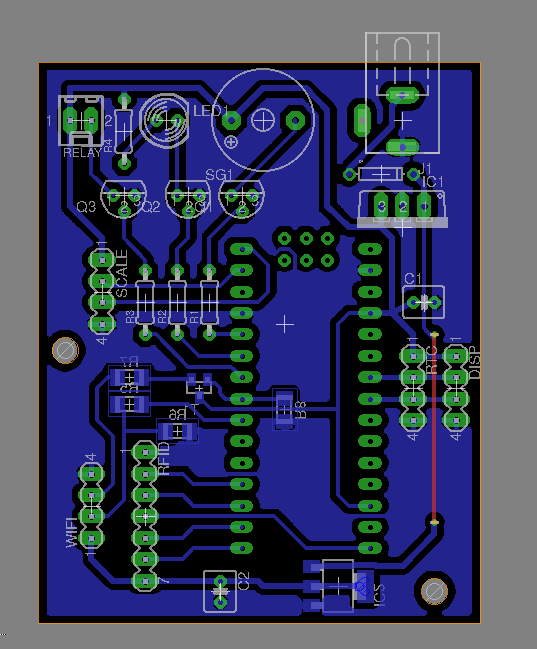
\includegraphics[width=0.9\textwidth]{images/weightlogger_pcb}
\end{figure}

\subsection{Administrative Software}

The administration software requested will be developed in Ruby On Rails for easier/faster development times.

\end{document}
